\documentclass[10pt]{article}
\usepackage[utf8]{inputenc}
\usepackage[doublespacing]{setspace}
\usepackage{textcomp}
\usepackage{amsmath,amssymb,amsthm}
\usepackage{fancyhdr}
\usepackage{lastpage}
\usepackage[]{hyperref}
\usepackage[pdftex]{graphicx}
\usepackage{ctex}
\usepackage{booktabs}
\usepackage{subfigure}
\usepackage{titlesec}
\usepackage{listings}
\usepackage{enumerate}
\usepackage{bm}
\usepackage{float}
%\allowdisplaybreaks
\renewcommand{\contentsname}{\centerline{Contents}}
\pagestyle{fancy}
\author{D}
\def\name{D}
\lhead{Data Mining}
\chead{}
\rhead{\name}
\cfoot{-\space\thepage\space-}
\newtheorem{exer}{\bm{$Exercise$}}
\newtheorem{prob}{\bm{$Problem$}}
\newtheorem{bonus}{\bm{$Bonus\;Problem$}}
\newcommand{\tabincell}[2]{\begin{tabular}{@{}#1@{}}#2\end{tabular}}
\CTEXoptions[today=old]

\begin{document}

\title{Assignment One}
\date{\today}
\maketitle
\thispagestyle{fancy}
\thispagestyle{fancy}

\begin{prob}
\end{prob}
\vspace{3mm}

a) One advantage of flexible approaches for regression is its permitting the modeling of nonlinearity, non-normal errors, and heteroskedasticity.\footnote{ Rust, R. T. (1988). Flexible regression. \textit{Journal of Marketing Research}, 25(1). 20.}\\

b) One disadvantage of flexible approaches for regression is its limitations in nominal and ordinal data, situations in which the variables are bounded or otherwise constrained, and addressing the dimensionality.\footnote{ Rust, R. T. (1988). Flexible regression. \textit{Journal of Marketing Research}, 25(1). 20.}\\

c) A less flexible approach is preferred in the conditions that the number of predictors is large, the sample size is small, and the variance of the errors is large.\footnote{ Lang, G. (2014). \textit{When does a flexible model beat an inflexible one and vice versa}. Retrieved from https://masterr.org/da/when-does-a-flexible-model-beat-an-inflexible-one-and-vice-versa/.}
\vspace{3mm}

\begin{prob}
\end{prob}
\begin{enumerate}[1)]
\vspace{3mm}

\item
R codes:
\lstinputlisting{p21a.R}
\begin{figure}[H]
  \centering
  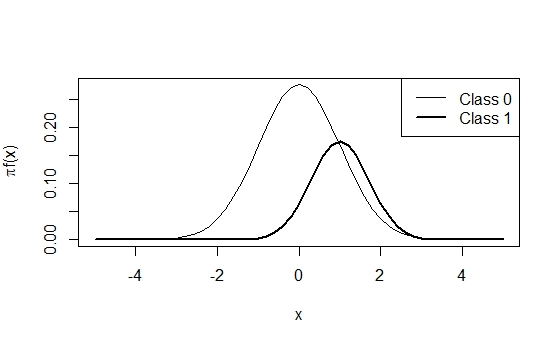
\includegraphics[width=8cm,height=5cm]{p21a.jpeg}
  \caption{$\pi_0f_0(x)$ and $\pi_1f_1(x)$} % Comment: Title? Color?
\end{figure}

\item
We have
\begin{equation}
\pi_0f_0(x)=\pi_1f_1(x).
\end{equation}
Using substitution and simplifying, we have
\begin{align*}
\frac{0.69}{\sqrt{2\pi}}e^{-\frac{1}{2}x^2}=\frac{0.31}{\sqrt{\pi}}e^{-(x-1)^2}.\\
\end{align*}
Solve the equation for x. We get
\begin{align*}
x\approx0.9546\;or\;3.0454.
\end{align*}
Hence, we get the Bayes boundary with values of 0.9546 and 3.0454.
\vspace{3mm}

\item
When $X=3$, the observation should be classified in Class 1, for $0.9546<x<3.0454$.
\begin{proof}
We test $X=3$ with $\pi_0f_0(x)$ and $\pi_1f_1(x)$ respectively.
\begin{align*}
\pi_0f_0(3)&=\frac{0.69}{\sqrt{2\pi}}e^{-\frac{1}{2}3^2}\\
&\approx0.0044\\
\pi_1f_1(3)&=\frac{0.31}{\sqrt{\pi}}e^{-(3-1)^2}\\
&\approx0.0103
\end{align*}
We get $\pi_0f_0(3)<\pi_1f_1(3)$.\\
According to the Bayes classifier, we have
\begin{equation}
f(x)=y_k,\;if\;P(Y=y_k|X=x)=\max_{y_j\subset C}P(Y=y_j|X=x).
\end{equation}
Hence, when $X=3$, the observation is classified in Class 1.
\end{proof}
\vspace{3mm}

\item
\begin{align*}
&P(an\;observation\;with\;X=2\;is\;in\;Class\;1)\\
&=\frac{P(X\;is\;in\;Class\;1|X=2)}{P(X\;is\;in\;Class\;0|X=2)+P(X\;is\;in\;Class\;1|X=2)}\\
&=\frac{\pi_1f_1(2)}{\pi_0f_0(2)+\pi_1f_1(2)}\\
&\approx\frac{0.2076}{0.0540+0.2075}\\
&\approx0.7936
\end{align*}
Hence, the probability that an observation with $X=2$ is in Class 1 is 0.7936. % Comment: 0.6333
\end{enumerate}
\vspace{3mm}

\begin{prob}
\end{prob}
\begin{enumerate}[1)]
\vspace{3mm}

\item
R codes:
\lstinputlisting{p31a.R} % Comment: Expecting to see MSE values for Training & Test Sets for all values of K
\vspace{3mm}

\item
We get the MSEs, when k = 2, 5, 10, 30, 50 and 100. Results in R:
\begin{align*}
&> mse(result\_2, y\_p)\\
&[1] 29.27373\\
&> mse(result\_5, y\_p)\\
&[1] 20.27732\\
&> mse(result\_10, y\_p)\\
&[1] 19.00983\\
&> mse(result\_30, y\_p)\\
&[1] 17.94852\\
&> mse(result\_50, y\_p)\\
&[1] 18.21337\\
&> mse(result\_100, y\_p)\\
&[1] 22.01719
\end{align*}
When k = 30, k performs the best with the smallest MSE.
\vspace{3mm}

\item
R codes:
\lstinputlisting{p33a.R}
\begin{figure}[H]
  \centering
  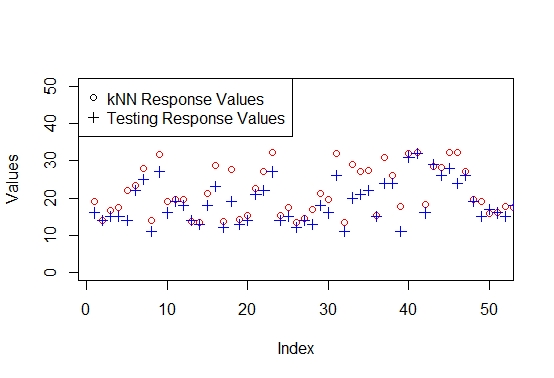
\includegraphics[width=8cm,height=5cm]{p33a.jpeg}
  \caption{kNN response values and testing response values} % Comment: Title? kNN model plot for all values of X
\end{figure}
After observing the plots with six given k values, we find the best fitness when k = 30. The graph shows that the kNN response values are close to the test response values when they are gathered, whereas they don't perform well for the dispersed values. In addition, many kNN response values look slightly larger than the corresponding test response values.
\vspace{3mm}

\item
We want to define a neighborhood for kNN regression to make both the bias and variance low. In other words, the response values by regression are close to the testing values. However, this is not always the case. We need to put the bias-variance trade-off in mind. High bias and low variance make the response values by regression gathered but away from the group of testing response values; low bias and high variance make the response values by regression centering around the group of testing response values but dispersed.\footnote{ Fortmann-Roe, S. (2012). \textit{Understanding the bias-variance tradeoff }. Retrieved from http://scott.fortmann-roe.com/docs/BiasVariance.html.} % Comment: large k -> high bias, low variance; small k -> low bias, high variance
\begin{figure}[H]
  \centering
  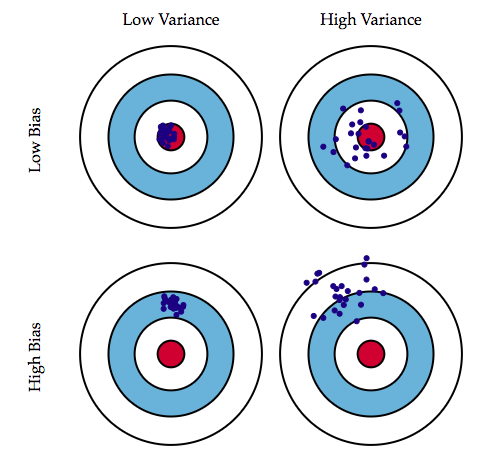
\includegraphics[width=6.5cm,height=6.5cm]{p34a.png}
  \caption{Graphical illustration of bias and variance}
\end{figure}

\vspace{3mm}
\end{enumerate}
\vspace{3mm}

\end{document}